The analysis of the distribution of seasonal events in Figure Figure~\ref{covid_heatmap} reveals a significant shift in the timing of the competition calendar. In 2020, there were more events in the second half of the year, indicating a clear departure from the traditional peak in midsummer. This shift towards late summer and autumn is still partially evident in 2021, although the calendar shows a gradual return to the pre-pandemic seasonal norm.

The Mann-Whitney-U test confirms a significant decline in performance levels across all athletic categories during the 2020 season compared to the 2015–2019 baseline ($p < 0.05$). The overall median IAAF score decreased by $-2.14\%$, falling from $935$ to $915$ points. Throws saw the largest decline ($-2.84\%$), followed by Jumps ($-2.45\%$) and Sprints ($-1.94\%$), while Runs remained most resilient ($-0.85\%$). 

The bootstrap analysis of the Interquartile Range (IQR) reveals significant shifts in performance dispersion during the 2020 season compared to the 2015--2019 baseline. Bootstrap analysis revealed significant increases in performance dispersion for Sprint ($+12.04\%$) and Run ($+6.41\%$), while the other disciplines Throw, Jump and remained statistically stable.

\begin{figure}[htb]
\vskip 0.2in
\begin{center}
\centerline{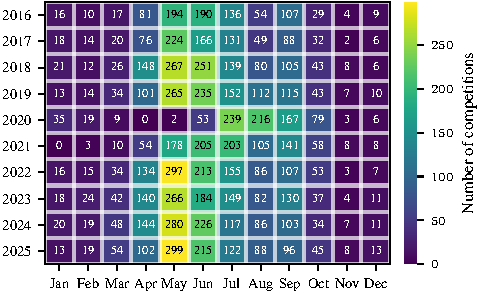
\includegraphics[width=\columnwidth]{figures/COVID_Heatmap_half.pdf}}
\caption{}
\label{covid_heatmap}
\end{center}
\vskip -0.2in
\end{figure}

\begin{figure}[htb]
\vskip 0.2in
\begin{center}
\centerline{
\includegraphics[width=\columnwidth]{figures/covid_relative_performance_change_half_baseline.pdf}}
\caption{}
\label{covid_relative_performance_change}
\end{center}
\vskip -0.2in
\end{figure}